\apendice{Anexo de sostenibilización curricular}

El desarrollo sostenible es un conjunto de principios aprobados en 2015 por la Organización de las Naciones Unidas (ONU), y recogidos en la Agenda 2030. La Agenda 20230 para el Desarrollo Sostenible es un plan de acción a nivel global, actualmente respaldada por los 193 países que pertenecen a la ONU, a favor de las personas, el planeta y las prosperidad económica, sanitaria y social, que además aboga por la paz universal y el acceso a la justicia\cite{Agenda2030_gobierno}

El desarrollo sostenible es considerado una oportunidad de mejora en la calidad de vida de todos los ciudadanos, sin excluir a nadie. Esto implica, entre otros objetivos, erradicar la pobreza, poner fin a todas las guerras, fomentar el acceso a una educación de calidad, adecuada y universal, garantizar unos servicios sanitarios universales, eficaces y de calidad, promover ciudades y comunidades inclusivas, seguras, resilientes y sostenibles. Para cumplir con todos los objetivos requieren de la cooperación de instituciones y gobiernos que aseguren mediante leyes e impulsos el cumplimiento y colaboración por parte de la sociedad.\cite{ODS}

Está formado por 17 Objetivos de Desarrollo Sostenible (ODS), cada uno con metas concretas cuyos objetivos deben alcanzarse antes del año 2030. En la \textit{Figura} \ref{fig:ODS}, se exponen cada uno de estos ODS.

\begin{figure}
\centering
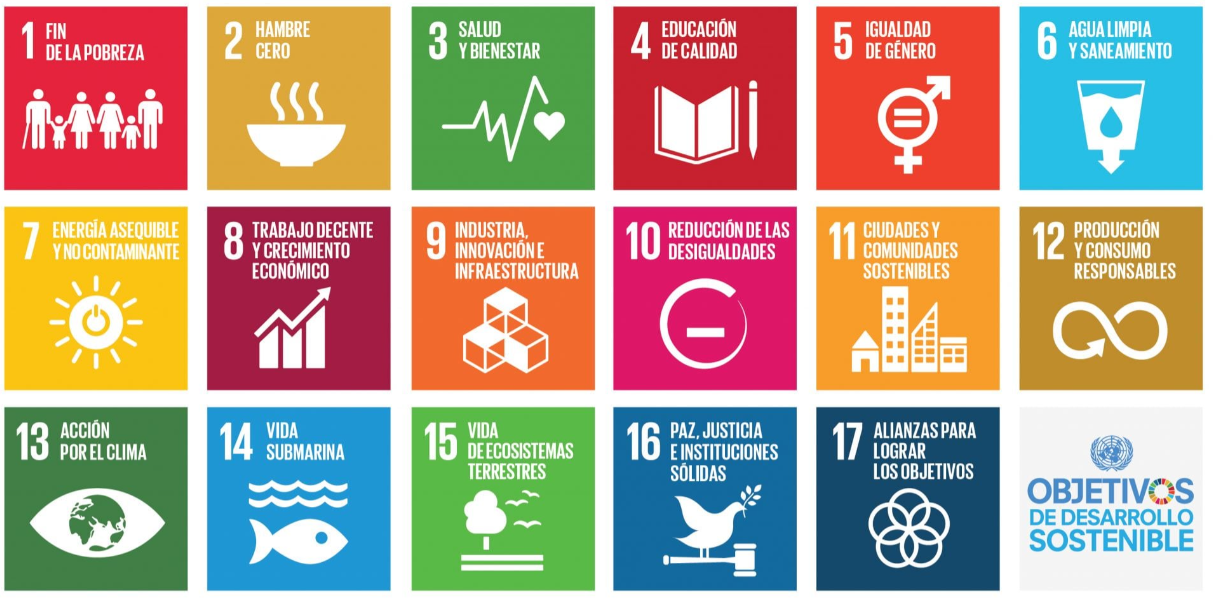
\includegraphics[width=1\linewidth]{img/ODS.png}
\caption{17 ODS. Fuente: un.org}
\label{fig:ODS}
\end{figure}

Dentro del desarrollo de este proyecto, se han identificado tres ODS particularmente relacionados, ya que la creación de un dispositivo de medición de la fuerza de los dedos y seguimiento puede contribuir con los objetivos marcados en la Agenda 2030, no solo en términos tecnológicos, sino también sociales y sanitarios.

En primer lugar, el ODS 3: Salud y Bienestar, cobra especial relevancia. Este objetivo busca el acceso universal a servicios sanitarios, garantizar una vida sana y promover el máximo bienestar posible para todas las personas y en todos los rangos de edades. El dispositivo y app desarrollados en este proyecto tiene como finalidad facilitar el seguimiento y evaluación de los pacientes en rehabilitación de la mano, proporcionando una herramienta especialmente útil en contextos clínicos y terapéuticos. Su diseño desde el inicio se ha planteado con un enfoque versátil, accesible y de bajo coste, lo cual permite su implementación en distintos tipos de centros sanitarios, incluyendo aquellos con recursos limitados. De este modo, se promueve una atención sanitaria más equitativa, eficiente y adaptada a las necesidades individuales de cada paciente, favoreciendo la recuperación funcional.\cite{salud_ODS}

En segundo lugar, el proyecto se relaciona con el ODS 9: Industria, Innovación e Infraestructura, cuyo objetivo es construir infraestructuras resilientes, promover la industrialización sostenible y fomentar la innovación. La creación de un dispositivo médico funcional, accesible y basado en tecnologías emergentes representa una aportación directa a la innovación tecnológica aplicada a la salud. \cite{infraestructura_ODS}

Por último, el ODS 10: Reducción de las Desigualdades, también se ve reflejado en este trabajo. Este objetivo busca reducir la desigualdad en y entre los países, promoviendo y potenciando la inclusión social, económica y política de todas las personas, independientemente de su edad, género, condición física o situación económica. Los prototipos desarrollados pueden contribuir a la ampliación en el acceso a tecnologías de rehabilitación, permitiendo que personas con escasos recursos o con discapacidades físicas puedan beneficiarse de tratamientos más personalizados, medibles y eficaces. Además, la posibilidad de adaptabilidad del sistema permite su uso por parte un gran número de profesionales para usuarios con diferentes patologías, lo que lo hace especialmente útil.\cite{desigualdades_ODS}

En conclusión, la creación de estos prototipos supone una pequeña contribución al cumplimiento de los ODS. Proporcionando una nueva tecnología, que impulsa el crecimiento de la industria y ámbitos sanitarios, fomentando la inclusión y reduciendo desigualdades.